% ------------Abstract------------

% Set the title for the abstract
\renewcommand{\abstractname}{Abstract}

% Uncomment the following lines to use the colorful abstract or monochrome abstract

% \begin{abstract}
%     This project implements a time machine as required by \textit{COMP0000J Intro to Temporal Engineering}.
% \end{abstract}
%
% \begin{colorfulabstract}
%     This project implements a time machine as required by \textit{COMP0000J Intro to Temporal Engineering}.
% \end{colorfulabstract}
%
\begin{monochromeabstract}
    This project implements a time machine as required by \textit{COMP0000J Intro to Temporal Engineering}.
\end{monochromeabstract}

% --------------------------------

\question{}
Formulae for building this time machine.
\begin{enumerate}[label=(\alph*)]
    \item \textbf{Common Operations \& Fractions}
        \begin{align}
            x + y - z &= \frac{a}{b} \cdot \sqrt{c^2 + d^2} \\
            \sum_{i=1}^{n} x_i^2 &= \int_{0}^{\infty} e^{-t} \, dt = \lim_{x \to \infty} \frac{1}{x} \\
            \alpha + \beta &= \gamma \quad \Delta \theta \neq \pi \quad \lambda \in \mathbb{R} \\
        \end{align}
    \item \textbf{More Formulae}
        $$
            A = \begin{pmatrix} a & b \\ c & d \end{pmatrix}, \quad
            \det(A) = \begin{vmatrix} a & b \\ c & d \end{vmatrix} = ad - bc
        $$
        and
        $$
            f'(x) = \frac{df}{dx} = \frac{\partial f}{\partial x}, \quad
            \nabla \cdot \vec{F} = \frac{\partial F_x}{\partial x} + \frac{\partial F_y}{\partial y}
        $$
        $$
            A \cup B \cap C \subseteq \mathbb{N}, \quad x \in A \implies x \notin B, \quad \forall x \exists y
        $$
    \item Also let's write some inline formulae like $\sin(\theta) + \cos^2(\phi) = \log(x) + \ln(y) + \binom{n}{k}$.
\end{enumerate}

% Enable one page for one question with the following command
% \enablenewpage

% And stop this behavior with
% \disablenewpage

\question{Propositions, Theorems and Principles.}
You can put your propositions, theorems and principles.
\begin{proposition}
    Time is not fixed.
\end{proposition}

\begin{theorem}
    Time travel is possible.
\end{theorem}

\begin{principle}
    Time travel is dangerous.
\end{principle}

There are also some predefined boxes with classical colors where you can put your notes. 
\begin{greenbox}{Green Note}
    Temporal Engineering is the study of time travel and its implications. It is a very interesting field of study. There are abundant online resources available for learning temporal engineering.
\end{greenbox}

\begin{bluebox}{Blue Note}
    You can make a lot of money after becoming a temporal engineer. The average salary of a temporal engineer is \$100,000,000 per year.
\end{bluebox}

\begin{yellowbox}{Yellow Note}
    There are many types of temporal engineer, such as frontend time machine engineer, backend time machine engineer, and full-stack time machine engineer. You can also specialize in time machine design, time machine testing, or time machine maintenance. DevOps time machine engineer is also a popular choice.
\end{yellowbox}



\question{Coding Question.}
    This is the implementation of the controller code of the time machine.

\begin{lstlisting}[language=Python, caption=Time Machine Demo]
def time_machine_controller():
    # This is the controller code of the time machine
    print("Time machine controller is running...")
    print("Please enter the year you want to travel to:")
    year = input()
    print(f"Travelling to {year}...")
    print("Time machine has arrived at the destination.")
    print("ERROR: Time machine has malfunctioned.")
    print("ERROR: You are now stuck in the year 2099.")
    print("ERROR: GOOD LUCK!")
\end{lstlisting}

\question{}
Maybe you would like a binary tree. \par
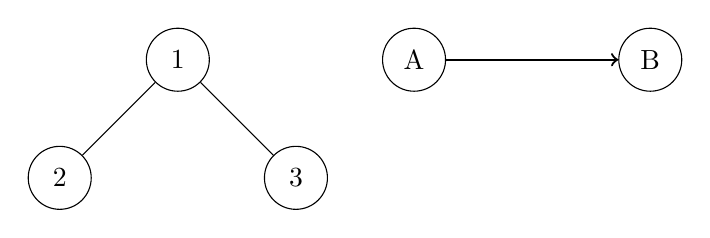
\begin{tikzpicture}[
  level distance=1.5cm,
  level 1/.style={sibling distance=3cm},
  level 2/.style={sibling distance=1.5cm},
  every node/.style={circle, draw, minimum size=0.8cm}
  ]
  \node {1}
    child {node {2}}
    child {node {3}};

  % Define nodes
  \node (A) at (3,0) {A};
  \node (B) at (6,0) {B};
  
  % Draw arrow from A to B
  \draw[->, thick] (A) -- (B);
\end{tikzpicture}

% You can also define your own numbering for the questions with the following command
\question*{}{12}
By running the \textit{Time Machine}, we jump to question 12 directly!

